\documentclass{standalone}

\usepackage{amsmath}
\usepackage{tikz}
\usetikzlibrary{decorations.pathreplacing, positioning}

\renewcommand{\familydefault}{\rmdefault}
\usepackage[T1]{fontenc}
\usepackage{lmodern}

\begin{document}

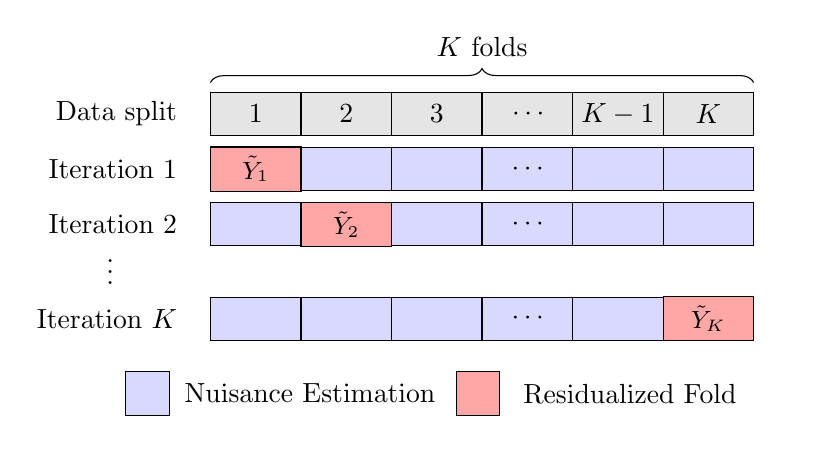
\begin{tikzpicture}[
    fold/.style={rectangle, draw=black, minimum width=1.15cm, minimum height=0.55cm},
    train/.style={fold, fill=blue!15},
    holdout/.style={fold, fill=red!35},
    split/.style={fold, fill=gray!20},
    label/.style={anchor=east},
]

% ---- Layout ----
\def\xstart{-0.2}
\def\w{1.15}
\def\ydata{0}
\def\yone{-0.7}
\def\ytwo{-1.4}
\def\ydots{-1.9}
\def\yk{-2.6}

% ---- Labels ----
\node[label] at (-0.5,\ydata) {Data split};
\node[label] at (-0.5,\yone) {Iteration 1};
\node[label] at (-0.5,\ytwo) {Iteration 2};
\node[label] at (-1.3,\ydots) {$\vdots$};
\node[label] at (-0.5,\yk) {Iteration $K$};

% ---- Header: K folds ----
\draw[decorate, decoration={brace, amplitude=5pt}]
    (\xstart,\ydata+0.4) -- ({\xstart+6*\w},\ydata+0.4)
    node[midway, above=6pt] {$K$ folds};

% ---- Data split row ----
\foreach \i/\lab in {0/1,1/2,2/3,3/$\hspace{2.3pt}\cdots$,4/$K-1$,5/$K$} {
    \node[split] at ({\xstart+\i*\w+\w/2},\ydata) {\lab};
}

% ---- Iteration 1 ----
\foreach \i in {0,...,5} {
    \ifnum\i=0
        \node[holdout] at ({\xstart+\i*\w+\w/2},\yone) {\small $\tilde Y_1$};
    \else
        \node[train] at ({\xstart+\i*\w+\w/2},\yone) {};
    \fi
}

% ---- Iteration 2 ----
\foreach \i in {0,...,5} {
    \ifnum\i=1
        \node[holdout] at ({\xstart+\i*\w+\w/2},\ytwo) {\small $\tilde Y_2$};
    \else
        \node[train] at ({\xstart+\i*\w+\w/2},\ytwo) {};
    \fi
}

% ---- Iteration K ----
\foreach \i in {0,...,5} {
    \ifnum\i=5
        \node[holdout] at ({\xstart+\i*\w+\w/2},\yk) {\small $\tilde Y_K$};
    \else
        \node[train] at ({\xstart+\i*\w+\w/2},\yk) {};
    \fi
}

% ---- Ellipsis inside rows ----
\node at ({\xstart+3.03*\w+\w/2},\yone) {$\cdots$};
\node at ({\xstart+3.03*\w+\w/2},\ytwo) {$\cdots$};
\node at ({\xstart+3.03*\w+\w/2},\yk) {$\cdots$};

% ---- Legend ----
\node[train, minimum width=0.55cm] at (-1,-3.55) {};
\node[right=0.15cm] at (-0.8,-3.55) {Nuisance Estimation};

\node[holdout, minimum width=0.55cm] at (3.2,-3.55) {};
\node[right=0.15cm] at (3.5,-3.55) {Residualized Fold};

\path[use as bounding box] (-1.0,-4.0) rectangle (7.3,0.8);

\end{tikzpicture}

\end{document}